\section{Funcionamiento}

La aplicación esta diseñada en 4 etapas, las cuales son mostradas en la Figura \ref{fig:procesoAppWeb}, donde la etapa \textbf{Selección} describe las secciones disponibles para obtener noticias; la etapa \textbf{Recolectar} muestra la integración de los \textit{crawlers} en la herramienta; la etapa \textbf{Clasificar} hace uso del modelo clasificador desarrollado en la sección anterior y para concluir, la etapa \textbf{Mostrar resultados} describe la forma en que los datos son presentados al usuario. A continuación se explica el funcionamiento de la aplicación.


\begin{figure}[H]
	\centering
	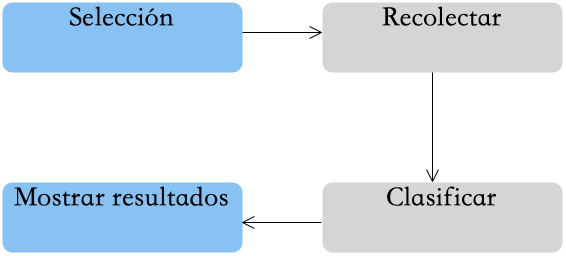
\includegraphics[scale=0.5]{imagenes/ProcesoAplicacionWeb.png}
	\caption{Etapas de la aplicación web}
	\label{fig:procesoAppWeb}
\end{figure}


\subsection{Selección}


La aplicación comienza en una pantalla inicial, donde se muestra un menú con las opciones \textbf{Inicio}, \textbf{Deportes}, \textbf{Economía}, \textbf{Cultura}, \textbf{Política}, \textbf{Ciencia y Tecnología}, estas categorías (excluyendo \textbf{Inicio}, la cual permite regresar a la pantalla principal) son las secciones permitidas para recolectar noticias, como se muestra en el Figura \ref{fig:PantallaInicio}. Como primer paso se debe dar click en una opción.\\


\begin{figure}[H]
\centering

\includegraphics[scale=0.35]{imagenes/pantallaPrincipal.png}
\caption{Pantalla de Inicio}
\label{fig:PantallaInicio}
\end{figure}

Después de elegir una sección, se muestra el mensaje \textbf{En proceso de recolección y clasificación}, como se visualiza en la Figura \ref{fig:loading}, el cual informa que las etapas \textbf{Recolectar} y \textbf{Clasificar} están en proceso, además cuando se muestra este mensaje no se puede seleccionar otra secciones hasta que el proceso haya concluido. Cabe destacar que el proceso continúa de forma normal si se cumplen las siguientes condiciones:

\begin{enumerate}
	\item \textbf{Primera vez}: Esta condición hace referencia a la etapa \textbf{selección}, es decir cuando es la primera vez que se ha selecciona una sección, se realiza la recolección de noticias

	\item \textbf{Límite de periodo}: Esta condición define 4 horas como el periodo de recolección, es decir cuando se ha solicitado mostrar las noticias de una sección y ha transcurrido 4 horas desde la última petición, se debe proceder con las siguientes etapas
\end{enumerate}	

Como consecuencia de no cumplirse estas condiciones, las etapas \textbf{Recolectar y Clasificar} no son iniciadas, debido a que los artículos con su clasificación correspondiente se encuentran almacenados en el sistema, por esta razón se procede directamente con la etapa \textbf{Mostrar resultado}.

\begin{figure}[H]
\centering
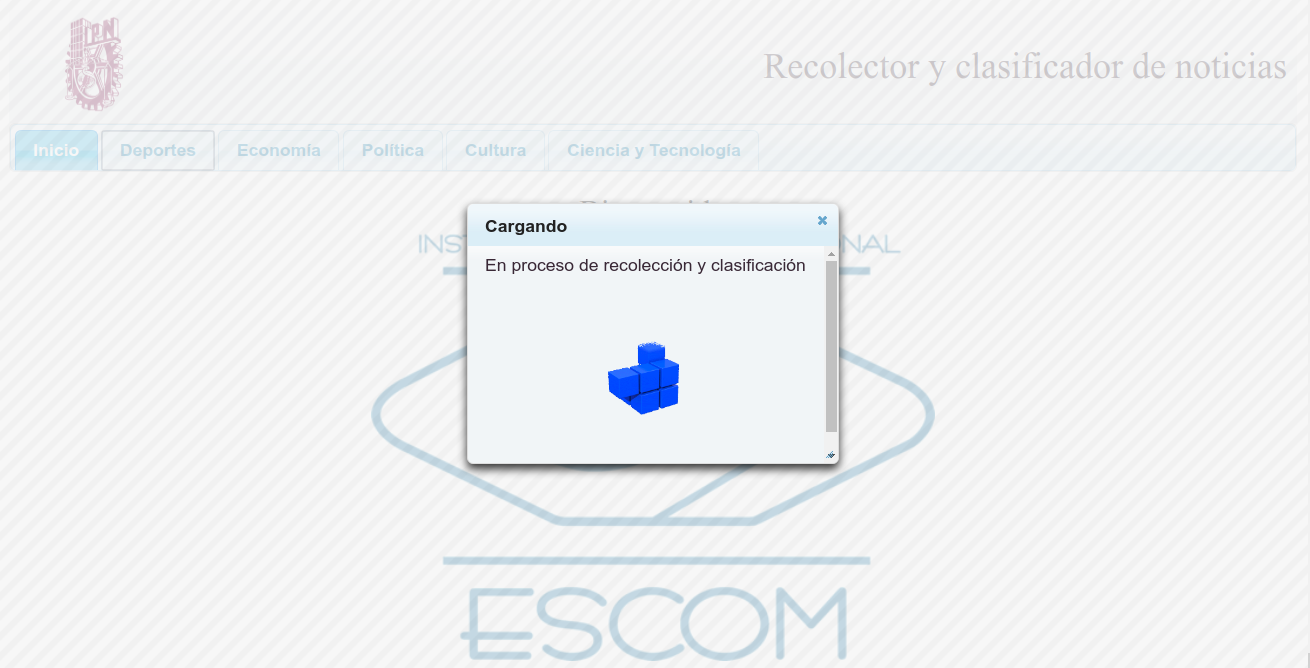
\includegraphics[scale=0.25]{imagenes/mensajeEspera.png}
\caption{Mensaje de espera}
\label{fig:loading}
\end{figure}


\subsection{Recolectar y clasificar}

La extracción de las noticias se hace en la página principal de los sitios web. Cabe destacar que en el proceso de recolección se valida que las noticias contengan al menos 180 palabras (en la redacción de \textbf{Noticia}), de lo contrario no se extrae. Ademas se ha definido un tiempo máximo de espera en esta etapa, el cual es de 30 segundos, después de concluir el periodo y haber recolectado la información, se procede con la etapa de \textbf{Clasificación}, de lo contrario si no se recolecto ninguna noticia se muestra el mensaje \textbf{Se ha agotado el tiempo de espera, no se han encontrado noticias, intentar mas tarde} (como se visualiza en la Figura \ref{fig:notNoRec}) y se detiene el proceso. Al concluir el proceso de recolección, las noticias obtenidas son clasificadas.

\begin{figure}[H]
\centering
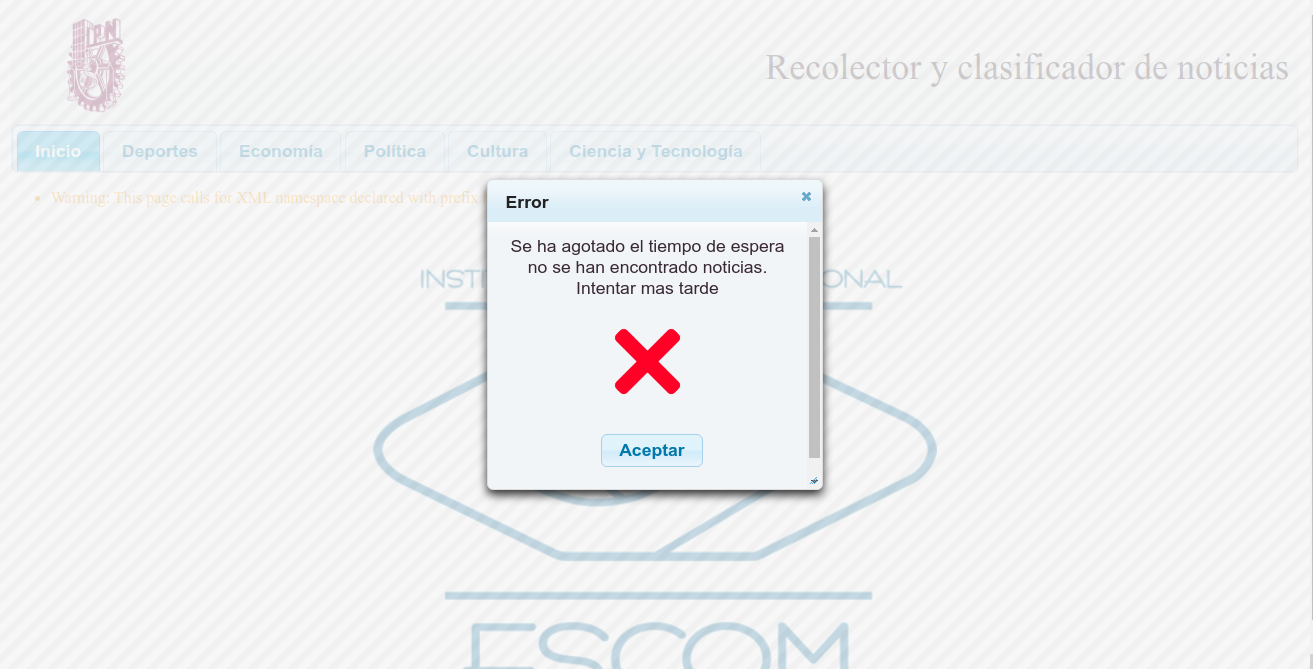
\includegraphics[scale=0.25]{imagenes/errorConectividad.png}
\caption{Mensaje de error en la recolección}
\label{fig:notNoRec}
\end{figure}


\subsection{Mostrar resultados}

Cuando el proceso de recolectar y clasificar ha concluido se muestra el mensaje \textbf{Noticias listas para ser mostradas}, donde se muestra la opción \textbf{Continuar}, la cual permite visualizar las noticias o la opción \textbf{cancelar}, como se muestra en la Figura \ref{fig:notClass}.

\begin{figure}[H]
\centering
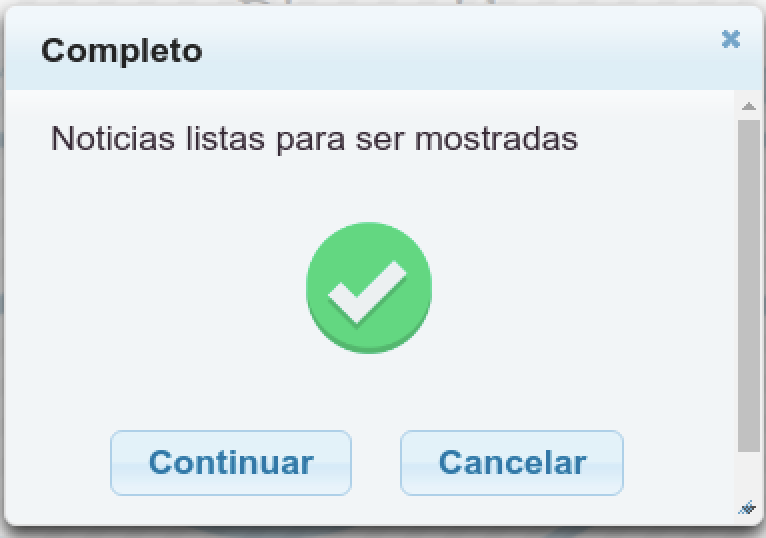
\includegraphics[scale=0.35]{imagenes/noticiasListasParaSerMostradas.png}
\caption{Mensaje que se muestra una vez clasificadas las noticias}
\label{fig:notClass}
\end{figure}

Si se ha presionado la opción \textbf{Cancelar}, el proceso concluye y la herramienta muestra la Pantalla de Inicio (ver \ref{fig:PantallaInicio}), de lo contrario si se ha dado clic en \textbf{Continuar}, se muestran las noticias en la aplicación, como se visualiza en la Figura \ref{fig:vistaNoticias}.


\begin{figure}[H]
\centering
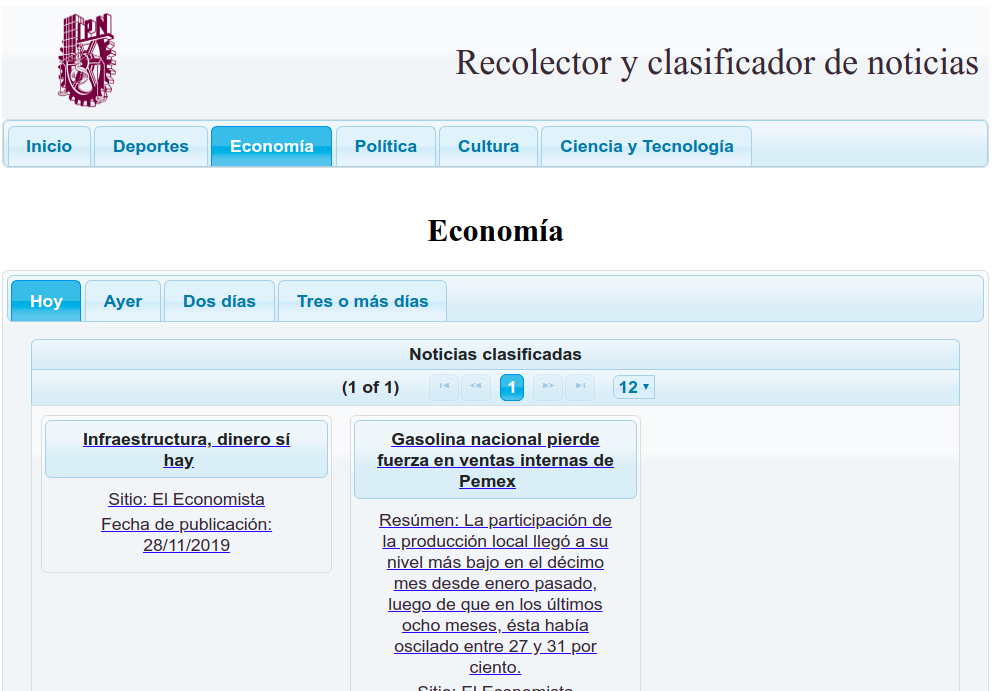
\includegraphics[scale=0.45]{imagenes/noticiasDeHoy.png}
\caption{Vista de las noticias recolectadas}
\label{fig:vistaNoticias}
\end{figure}



\subsection{Filtro fecha}

En la sección de las noticias, se muestra un menú con las opciones: \textbf{Hoy}, \textbf{Ayer}, \textbf{Dos días} y \textbf{Tres días o mas}. Este es una herramienta que permite filtrar los artículos por fecha de publicación. Por ejemplo, si se desea visualizar noticias de un día anterior a la registrada por el sistema, se debe seleccionar la opción \textbf{Ayer}, en seguida la información de este periodo se muestra, como en la Figura \ref{fig:vistaNoticiasAyer}. Es importante mencionar que las noticias mostradas por defecto son las del día de consulta (\textbf{Hoy}).



\begin{figure}[H]
\centering
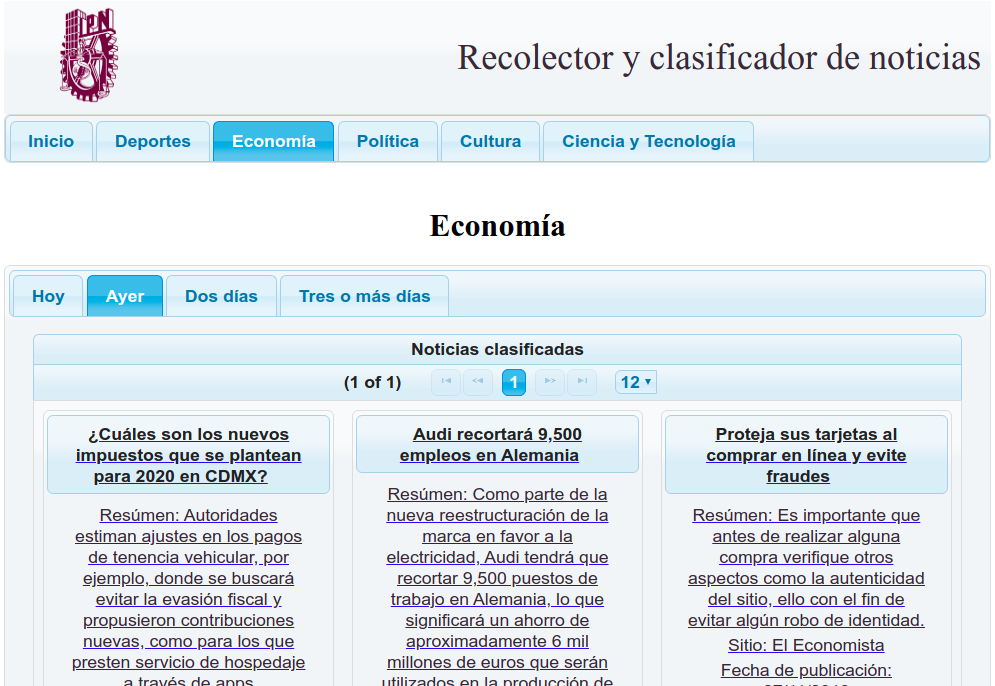
\includegraphics[scale=0.45]{imagenes/noticiasDeAyer.png}
\caption{Vista de las noticias recolectadas del día de ayer}
\label{fig:vistaNoticiasAyer}
\end{figure}


\subsection{Ingresar al sitio de origen}

Cada noticia mostrada contiene la \textbf{URL} ( de forma interna ) al sitio de origen de la noticia, si se requiere  leer el artículo completo se debe dar clic en la caja que contiene la noticia y la aplicación redirige el buscador al sitio fuente. Además, para regresar al recolector y clasificador, debe redirigirse nueva mente a la URL de la aplicación.

